% Koma-Klasse für ein Buch:
%  12pt Schriftgröße
%  A4 Seitenformat
%  Bibliography ins Inhaltzverzeichnis
%  Trennlinie für die Kopfzeile
%  kleine Überschriften (alternativ: normalheadings, bigheadings)
%  zweiseitiger Druck (alternativ: oneside)
%  Kapitel immer auf ungeraden Seiten beginnen
%  fleqn: abgesetzte mathematische Formeln sind linksbündig
%  "Anhang" wird vor die Kapitelüberschriften im Anhang gesetzt (chapterprefix hat den gleichen Effekt für normale Kapitel)
%  BCORXmm reserviert X mm zusätzlichen Rand für die Bindung
\documentclass[12pt,a4paper,bibtotoc,headsepline,smallheadings,twoside,openright,fleqn,appendixprefix,BCOR=5mm]{scrbook}

\usepackage[utf8]{inputenc}
%\usepackage[ansinew]{inputenc} % Zeichenkodierung
\usepackage[T1]{fontenc} % Trennung von Wörtern mit Umlauten
%\usepackage{eurofont} %Das Euro-Zeichen
\usepackage{lmodern} % Latin Modern font benutzen (enhanced computer modern clone, serif)
%\usepackage{tgpagella} % TeX Gyre Pagella font benutzen (palatino clone, serif)
%\usepackage{tgtermes} % TeX Gyre Termes font bentzen (times clone, serif)
\usepackage[ngerman]{babel} % Dokumnt in deutsch inklusive Silbentrennung nach neuer deutscher Rechtschreibung
%\usepackage[UKenglish]{babel} % Englische Sprachunterstützung (alternativ: USenglish)
\usepackage{natbib} % Stil für Literaturverzeichnis
\usepackage{amsmath} % verbesserte mathematische Umgebung
\usepackage{amsfonts} % zusätzliche mathematische Zeichen
\usepackage{amssymb} % zusätzliche mathematische Zeichen
\usepackage{amsthm} % zusätzliche mathematische Zeichen
\usepackage{exscale} % Anpassung mathematischer Symbole an die Schriftgröße
\usepackage{amstext} % \text in mathematischer Umgebung
\usepackage{array} % Tabellen
\usepackage{multirow}
\usepackage[table,xcdraw]{xcolor}
\usepackage{rotating} % rotierte Tabellen und Bilder
\usepackage[ruled, german]{algorithm2e} % Pseudocode
\usepackage{verbatim} % Funktion zum Schreiben von unformatiertem Text
\usepackage{float} % Ermöglicht das Erstellen von eigenen Float Umgebungen
\usepackage[section]{placeins} % Verhindert das Wandern von floats in eine andere section
\usepackage{color} % Farbiger Text
\usepackage{graphicx} % Funktionen zum Einfügen von Bildern
\usepackage{subfigure} % Anzeigen von Bildern aus mehreren Einzelbildern
\usepackage{setspace} % Einstellen des Zeilenabstandes
\usepackage[plainpages=false,pdfpagelabels=true,colorlinks=true,linkcolor=black,citecolor=black,bookmarksopen=true]{hyperref} % Verweise werden im PDF zu Hyperlinks
\usepackage{scrpage2} % Koma für Kopfzeilen-Formatierung

\bibliographystyle{dinat} % Literaturverzeichnis entsprechend DIN 1505 formatiert
\renewcommand{\topfraction}{0.85} % Anteil einer Seite, die von Floats belegt sein darf (default 0.7)
\renewcommand{\textfraction}{0.1} % Anteil einer Seite, die mindestens Text sein muss (default 0.2)
\renewcommand{\floatpagefraction}{0.75} % Anteil einer Seite, die ein Float einnehmen darf, ohne auf die nächste Seite gesetzt zu werden (default 0.5)
\singlespacing % Zeilenabstand setzen (alternativ: onehalfspacing, doublespacing)
\definecolor{grey}{gray}{0.5}
\newcommand{\todo}[1]{
	% Die folgende Zeile kann auskommentiert werden, um die ToDo's zu entfernen
	\textcolor{red}{[\textbf{ToDo}: \emph{#1}]}
}
\newcommand{\note}[1]{
	% Die folgende Zeile kann auskommentiert werden, um die Notes zu entfernen
	\textcolor{grey}{[\textbf{Anmerkung}: \emph{#1}]}
}
\newcommand{\argmax}{\operatornamewithlimits{argmax}}
\newcommand{\argmin}{\operatornamewithlimits{argmin}}

\begin{document}

\pagestyle{empty}
\pagenumbering{alph}
\begin{titlepage}
\begin{figure}[H]
\centering
	
\includegraphics[scale=0.4]{fotos/misOR}
\end{figure}
\begin{center}
MisOR\\
Fachgebiet Wirtschaftsinformatik, insb. Operations Research \\
Fakultät Wirtschaftswissenschaften\\
Universität Paderborn\\     
\vspace{8ex}
\Large
Masterarbeit\\
\vspace{8ex}
\textbf{\sffamily{Heuristische Lösungsansätze\\zur Optimierung des Routenplans\\ mit Sendungskonsolidierung\\}}
\vspace{6ex}
\normalsize
von\\
Ahmad Hashemi\\
6785702\\
Bieberer Straße 27\\
63065 Offenbach am Main\\
haschemi.ahmad@gmail.com\\
\vspace{8ex}
vorgelegt bei\\
Prof. Dr. Guido Schryen\\
\normalsize
\vspace{16ex}
\today
\end{center}
\end{titlepage}
 % Titelblatt
\cleardoublepage

\section*{\centering Sperrvermerk}

\noindent\textbf{verlangter Sperrvermerk von DB:}\\
Die nachfolgende Masterarbeit mit dem Titel „Heuristische Lösungsansätze zur Optimierung des Routenplans mit Sendungskonsolidierung“ \todo{Titel} enthält vertrauliche Daten der Deutschen Bahn AG. Veröffentlichungen oder Vervielfältigungen der Masterarbeit - auch nur auszugsweise - sind ohne vorherige ausdrückliche Zustimmung der Deutschen Bahn AG nicht gestattet. Die Masterarbeit ist nur Korrektoren sowie den Mitgliedern der Prüfungskommission zugänglich zu machen. \\
\\
Ort/Datum: \hrulefill\quad Unterschrift: \hrulefill\\

%\noindent\textbf{Vom Diplomanden zu unterschreiben:}\\
%Die Diplomarbeit wurde im Rahmen eines laufenden Projektes bei der <Firmenname> durchgeführt. Um eine Geheimhaltung\footnote{Bei Wegfall des Geheimhaltungserfordernisses ergeht eine gesonderte Information an Diplomand und Fakultät.} zu gewährleisten, verpflichte ich mich - von Beginn bis mindestens für 5 Jahre nach Abgabe der Diplomarbeit - Veröffentlichungen jeglicher Art der Diplomarbeit oder ihres wesentlichen Inhalts nicht vorzunehmen. Aus diesem Grund muss auch eine Aufnahme eines Exemplars der Diplomarbeit zur Einsicht und Ausleihe in der Bibliothek der Universität Paderborn während des genannten Zeitraums unterbleiben.\\
%Ich habe keine Einwände, dass das Thema meiner Diplomarbeit mit meiner Namensnennung in einem Verzeichnis der Hochschule genannt wird.\\
%\\
%Ort/Datum: \hrulefill\quad Unterschrift: \hrulefill\\
%\\
%\\
%\textbf{Von der Fakultät Wirtschaftswissenschaften der Universität Paderborn zu unterschreiben:}\\
%Aus den oben genannten Gründen verpflichtet sich die Fakultät entsprechend, Veröffentlichungen der Diplomarbeit oder ihres wesentlichen Inhalts nicht vorzunehmen und die Diplomarbeit auch nicht zur Einsicht und Ausleihe in die Bibliothek aufzunehmen.\\
%\\
%Ort/Datum: \hrulefill\quad Unterschrift: \hrulefill\\
%\\
%\\
%\textbf{Vom Betreuer der <Firmenname> zu unterschreiben:}\\
%Oben genannter Sperrvermerk zur Kenntnis genommen.\\
%\\
%Ort/Datum: \hrulefill\quad Unterschrift: \hrulefill
 % Sperrvermerk, falls die Arbeit in Kooperation mit einer Firma entstanden ist und vertrauliche Firmendaten enthält
\cleardoublepage

\noindent
Hiermit erkläre ich an Eides Statt, dass ich die vorliegende Arbeit selbständig und ohne unerlaubte fremde Hilfe angefertigt, andere als die angegebenen Quellen und Hilfsmittel nicht benutzt und die den benutzten Quellen und Hilfsmitteln wörtlich oder inhaltlich entnommenen Stellen als solche kenntlich gemacht habe.\\
\\
\\
Paderborn, \today
\begin{flushright}
------------------------------------------\\
(Vorname Name)
\end{flushright} % eidesstattliche Erklärung
\cleardoublepage

\section*{Abstract - deutsch}
Eine Zusammenfassung der Arbeit in deutscher Sprache.
\\
\textbf{Stichworte:} ...

\section*{Abstract - englisch}
Eine Zusammenfassung der Arbeit in englischer Sprache.
\\\\
\textbf{Keywords:} ...
\\\\\\
\note{Diese Vorlage ist für zweiseitigen Druck gemacht, kann aber durch eigene Anpassungen auch für den einseitigen Druck benutzt werden. Welche Anpassungen das sind, kann der Standardliteratur zu \LaTeX{} entnommen werden (siehe dazu \ttfamily{docs/}).} % Abstract
\cleardoublepage

\pagestyle{scrheadings}
\frontmatter
\tableofcontents % Inhaltsverzeichnis
\cleardoublepage

\listoffigures % Abbildungsverzeichnis
\cleardoublepage

\listofalgorithms % Liste der Algorithmen
\cleardoublepage

\listoftables % Tabellenverzeichnis
\cleardoublepage

\newfloat{ergebnisse}{thb}{loh}[chapter] % Liste der detaillierten Ergebnisse
\floatname{ergebnisse}{Ergebnisse}
\listof{ergebnisse}{Liste der detaillierten Ergebnisse}
\cleardoublepage

\mainmatter % der eigentliche Text folgt hier
\chapter{Einleitung}
In diesem Kapitel werden die relevanten Konzepte des Schienengüterverkehrs im Zusammenhang mit unserer Problemstellung vorgestellt, wobei nach einer kurzen Einführung die Hintergrundauskünfte und Terminologie im Unterabschnitt \hyperref[sec:problem]{1.1.1} erklärt werden. Es folgt eine ausführliche Problemdarstellung im Unterabschnitt \hyperref[sec:discription]{1.1.2} , und eine Zusammenfassung des aktuellen Lösungsansatzes im Unterabschnitt \hyperref[sec:current]{1.1.3}.\\
Schließlich wird im Abschnitt \hyperref[sec:Ziel]{1.1.2} das Ziel dieser Abschlussarbeit bezüglich der beschriebenen Problematik im vorherigen Abschnitt verdeutlicht.

\section{Problematik}
\label{sec:problem}
In langfristiger Hinsicht nimmt Güterverkehr bei globalisierten Märkten zu, und Deutschland als zentrale Verkehrsverbindung spielt eine wichtige Rolle in Logistik von Europa. DB Cargo ist ein führender globaler Logistikdienstleister und der größte Anbieter im Schienengüterverkehr in Europa. Schienenverkehr ist eine ökonomische und umweltfreundliche Form der Transportation. Es dient zur Verteilung der sowohl schweren Container wie Massengüter von Kohlen oder Stahl als auch kleineren Sendungen, die nur einen Teil des gesamten Zugs besetzen. Entwurf eines Verwaltungssystems zur Fahrplanung und Konsolidierung der Sendungen unter minimierten Kosten ist jedoch eine große Herausforderung.

\todo{absprechen} DB Schenker ist ein führender globaler Anbieter der Logistikdienstleistungen, der weltweit Industrie und Handel beim Güteraustausch durch Landverkehr, Luft- und Seefracht, Kontraktlogistik und Supply Chain Management unterstützt. Mit 430 Standorten für den europaweiten Landverkehr ermöglicht DB Schenker Güterströme zwischen beiden Verkehrsträgern (bzw. auf der Straße oder Schiene) in einem umfassenden Netzwerk. Damit verbindet er die besonderen Vorteile der einzelnen Transportarten durch innovative multimodale Lösungen, um die Sendungen termingerecht mit höherer Flexibilität zu transportieren. Entwurf eines Verwaltungssystems zur Fahrplanung und Konsolidierung der Sendungen unter minimierten Kosten ist jedoch eine große Herausforderung.

\subsection{Problemspezifische Begriffe und Parameter}
Um die Problemdarstellung besser nachzuvollziehen und die Parameter des Modells kennenzulernen, wird im folgenden Unterabschnitt die notwendige technische Terminologie aus dem Güterverkehrssystem sowie deren Parameter dargestellt.

\subsubsection{Wagen}
Ein Wagen ist eine meist vierrädrige Ladeeinheit zum Beladen der Güter und bezeichnet die kleinste Transporteinheit. Er verfügt üblicherweise über keinen Antrieb, deswegen wird eine Kupplung der Wagen mit einer Lokomotive gezogen. Es gibt verschiedene Arten von Güterwagen, die je nach Güterformen spezifiziert worden sind. Bei dieser Arbeit wurden die Wagen jeder Sendung als gleich angenommen. Die Wagen verschiedener Sendungen können jedoch unterschiedliche Kosten verursachen.

\subsubsection{Anlagen (Bahnhöfe)}
Eine Anlage in Bezug auf Schienengüterverkehr ist eine Station (ein Bahnhof), wo die Güter ein- bzw. ausgeladen oder die Wagen zur Erstellung eines neuen Zugs umrangiert werden.\\
Folgende Tabelle zeigt die Parameter, die eine Anlage kennzeichnen.

\begin{table}[ht]
\centering
\begin{tabular}{lll}
\hline
\rowcolor[HTML]{000000} 
{\color[HTML]{FFFFFF} } & {\color[HTML]{FFFFFF} \textbf{Beschreibung}}                                           & {\color[HTML]{FFFFFF} \textbf{Parameter}} \\ \hline
\textbf{1}                   & \begin{tabular}[c]{@{}l@{}}Max. Anzahl der Wagen, die in Anlage $i$ umgestellt\\ werden \end{tabular}                           & MaxWagonCount          \\ 
\hline
\multirow{2}{*}{\textbf{2} } & \multirow{2}{*}{Max. Anzahl der ein- bzw. ausgehenden Züge an Anlage $i$}                                                       & MaxIngoingTrainCount   \\
                             &                                                                                                                               & MaxOutgoingTrainCount  \\ 
\hline
\multirow{2}{*}{\textbf{3} } & \multirow{2}{*}{\begin{tabular}[c]{@{}l@{}}Max. Anzahl der ein- bzw. ausgehenden Richtungsgleise\\ an Anlage $i$ \end{tabular}} & MaxOutgoingTrackCount  \\
                             &                                                                                                                               & MaxIngoingTrackCount   \\ 
\hline
\textbf{4}                   & Die Fixkosten der Anlage $i$                                                                                                   & FixedCosts             \\ 
\hline
\textbf{5}                   & Umstellkosten der Anlage $i$                                                                                                    & SwithCosts            \\
\hline
\textbf{6}                   & Die kosten der ausgehendenRichtungsgeleise der Anlage $i$                                                                                                    & OutgoingTrackCosts 
\end{tabular}
\caption{Liste der Parameter einer Anlage}
\end{table}

Die Kosten einer Anlage sind im Fall der Umstellung relevant, und bestehen aus drei Kostenkomponenten, nämlich den Fixkosten der Anlage, den Kosten der ausgehenden Richtungsgeleise und den Umstellkosten. Die Anlagenfixkosten verursachen einen Pauschalwert, falls die Anlage mindestens einmal in einer Sendungsroute vorkommt. Die Umstellkosten sind jedoch linear pro Sendungseinheit zu berechnen.

\subsubsection{Kanten}
Eine Kante verbindet zwei Anlagen und kann einer Sendungsmenge oder den Wagen zugeordnet werden. Die einer Kante zugeordneten Wagen fahren zu einer gewissen Abfahrtszeit gemeinsam  zum Endknoten der Kante, ohne zwischendurch umgestellt zu werden. Sie werden in mehrere Züge aufgeteilt, falls die Länge- oder Gewichtskapazität eines Zuges überschritten wird. Es ist folglich erlaubt, dass mehr als ein Zug gleichzeitig auf einer Kante fahren. Maximale Anzahl der fahrenden Zügen auf einer Kante ist aber eingeschränkt.\\
Die auf einer Kante fahrenden Wagen können verschiedene Zielknoten oder Pfade haben , d.h. verschiedene Sendungen können gemeinsam auf einer Kante fahren. Die Trennung einer Sendung in zwei oder mehr Kanten ist jedoch nicht erlaubt. \\
Die Parameter einer Kante sind in der folgenden Tabelle aufgelistet.

\begin{table}[ht]
\begin{tabular}{lll}
\hline
\rowcolor[HTML]{000000} 
{\color[HTML]{FFFFFF} } & {\color[HTML]{FFFFFF} \textbf{Beschreibung}}                                           & {\color[HTML]{FFFFFF} \textbf{Parameter}} \\ \hline
\textbf{1}              & \begin{tabular}[c]{@{}l@{}}Max. zulässige Zuglänge auf Kante\\ (i, j)\end{tabular}     & MaxLength                                 \\ \hline
\textbf{2}              & \begin{tabular}[c]{@{}l@{}}Max. zulässiges Zugsgewicht\\ auf Kante (i, j)\end{tabular} & MaxWeight                                 \\ \hline
\textbf{3}              & \begin{tabular}[c]{@{}l@{}}reine Reisezeit für Zug von i\\ zu j\end{tabular}           & TravelTime                                \\ \hline
\textbf{4}              & Distanz zwischen i und j                                                               & Distance                                  \\ \hline
\textbf{5}              & \begin{tabular}[c]{@{}l@{}}Kosten für einen Zug auf Kante\\ (i, j)\end{tabular}        & CostPerTrain                              \\ \hline
\textbf{6}              & \begin{tabular}[c]{@{}l@{}}Ausgangsbearbeitungszeit von i\\ zum j\end{tabular}         & DepartureProcessingTime                   \\ \hline
\textbf{7}              & \begin{tabular}[c]{@{}l@{}}Umstellzeit für einen Zug in j\\ kommend von i\end{tabular} & ArrivalProcessingTime                     \\ \hline
\textbf{8}              & \begin{tabular}[c]{@{}l@{}}Die regulären Abfahrtszeiten\\ von i zum j\end{tabular}     & DepartureTime                             \\ \hline
\textbf{9}              & \begin{tabular}[c]{@{}l@{}}Max. Anzahl der Zügen\end{tabular}     & MaxTrainCount                             \\ \hline
\end{tabular}
\caption{Liste der Parameter einer Kante}
\end{table}

\subsubsection{Sendungen}
Eine Sendung bezieht sich auf eine Transportbestellung zwischen zwei Anlagen des Schienennetzes. Jede Sendung besteht aus einer bestimmten Anzahl Wagen und hat auch ein gewisses Gewicht und eine gewisse Länge. Für jede Sendung ist eine maximale Transportzeit anzugeben, d.h. jede Sendung soll innerhalb des Zeitraums von ihrer Aufkommenszeitpunkt in der Quelle bis zur Ankunftszeit am Ziel geliefert werden. In der folgenden Tabelle sind die Parameter einer Sendung aufgelistet.

\begin{table}[ht]
\begin{tabular}{lll}
\hline
\rowcolor[HTML]{000000} 
{\color[HTML]{FFFFFF} } & {\color[HTML]{FFFFFF} \textbf{Beschreibung}} & {\color[HTML]{FFFFFF} \textbf{Parameter}} \\ \hline
\textbf{1} & Quellanlage der Sendung k & StartId \\ \hline
\textbf{2} & Zielanlage der Sendung k & EndId \\ \hline
\textbf{3} & Länge der Sendung k & Length \\ \hline
\textbf{4} & Gewicht der Sendung k & Weight \\ \hline
\textbf{5} & Anzahl Wagen der Sendung k & WagonCount \\ \hline
\textbf{6} & Max. Transportzeit der Sendung k & MaxTransportTime \\ \hline
\textbf{7} & \begin{tabular}[c]{@{}l@{}}Kosten pro Wagen der Sendung k\\ pro Stunde vom Transport\end{tabular} & CostPerWagonHour \\ \hline
\textbf{8} & Aufkommenszeitpunkt der Sendung k & DepartureTime \\ \hline
\textbf{9} & Maximale Anzahl der Umstellungen & MaxSwitchCount \\ \hline
\textbf{10} & Strafkosten, falls Routen obligatorisch ist & PenaltyCosts \\ \hline
\textbf{12} & Umwegigkeitsfaktor & DetourFactor \\ \hline
\textbf{13} & Max. Distanz der Umwegigkeit & \begin{tabular}[c]{@{}l@{}}MaxAbsolute-\\ DetourDistance\end{tabular} \\ \hline
\end{tabular}
\caption{Liste der Parameter einer Sendung}
\end{table}

\subsubsection{Route und Routenplan}
\label{subsec:routenplan}
Für jede Sendung ist eine Route in einem Transportnetzwerk festzulegen, die aus einer Folge der Bahnhöfe besteht. Diese Reihenfolge beschreibt, an welchen Anlagen die Wagen umrangiert und zu neuen Zügen zusammengestellt werden. Eine Route jeder Sendung beginnt mit der Sendungsquelle, wird ggf. von den mittleren Anlagen sowie den Rangierbahnhöfen gefolgt, und endet mit dem Sendungsziel. Ein Routenplan eines Szenarios umfasst die Routen für jedes Paar von Quell- und Zielknoten jeder Sendung. Das Ziel besteht darin, ein Entscheidungsunterstützungssystem zu präsentieren, das den optimale Routenplan bzw. einen guten Routenplan innerhalb vorgegebener Rechenzeit oder akzeptable Lösungsqualität herausfindet.

\subsubsection{Konsolidierungseffekt}
Zum Verständnis der Wichtigkeit der Konsolidierung ist es zu berücksichtigen, dass die Fixkosten des Zugs beim Schienengüterverkehr (die Kosten für Lokomotive und Personal) die anderen Kostenkomponenten dominieren. Mit der Bündelung der Sendungen kann man die Züge mit möglichst voller Kapazität bzw. maximaler Anzahl der Wagen zu routen, und somit die Zugkosten zu verringern. Auf der anderen Seite verursacht die Konsolidierung aber andere Kosten wie längere Transportzeit und Umstellungskosten. Die Herausforderung besteht somit darin, unter Berücksichtigung der Kapazitäten und Einschränkungen den Kompromiss zwischen den gegensätzlichen Zielen zu finden. Bild 1 stellt drei mögliche Lösungsvarianten dar, die drei Sendungen jeweils vom Ziel zur zugehörigen Quelle transportieren. Beim Bild1(a) fahren die Sendungen auf den kürzesten Pfaden. Bei der Variante Bild1(b) wurde ein konsolidierter Ansatz angenommen. Das Bild1(c) stellt eine gemischte Lösung der vorherigen Ansätze dar. Welche der angebotenen Lösungen den besseren Zielfunktionswert aufweist, hängt von der Probleminstanz und der Parametereingabe ab. Auf jeden Fall kann ein Ansatz basierend auf kürzesten Pfade die Optimalität nicht gewährleisten.

\begin{figure}[ht]
\subfigure[kürzester Pfad]{\label{fig:a}
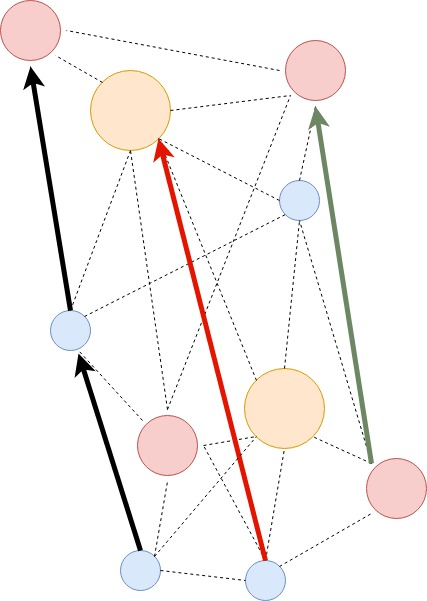
\includegraphics[scale=0.3]{fotos/shortestpath.jpg}}
\subfigure[konsolidierter Pfad]{\label{fig:b}
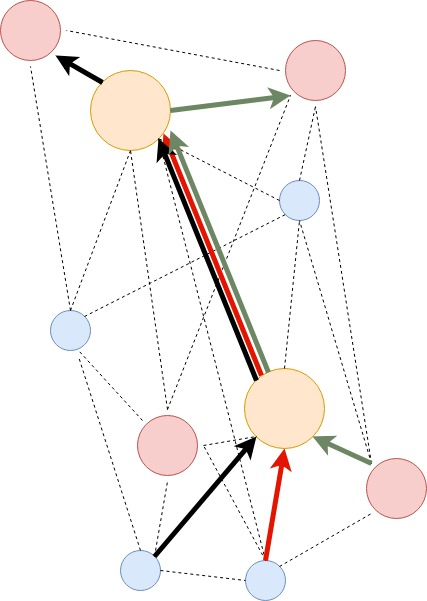
\includegraphics[scale=0.3]{fotos/cosolidated.jpg}}
\subfigure[gemischte Lösung]{\label{fig:c}
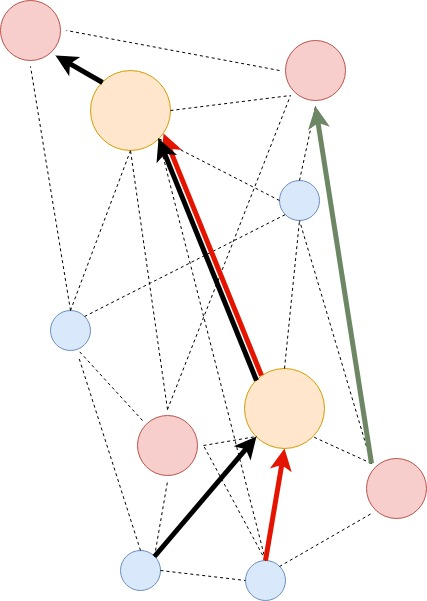
\includegraphics[scale=0.3]{fotos/mixedpath.jpg}}
\caption{Drei verschiedene Transportlösungen}
\end{figure}

\subsection{Problembeschreibung}
\label{sec:discription}
Die Modellierung eines Entscheidungsunterstützungssystems als ein Optimierungsproblem ist mit rechenbarem Ziel sowie Einschränkungen verbunden. Im folgenden Unterabschnitt wird die Nebenbedingungen sowie Zielfunktion des Modells konkret dargestellt.

\subsubsection{Nebenbedingungen}
In verschiedenen Szenarien (Probleminstanzen) gibt es verschiedene betriebliche Einschränkungen, deshalb soll der Anwender in der Lage sein, eine Kombination der Nebenbedingungen je nach Fragestellung auszuwählen.

\paragraph{Anzahl der Züge.}
Ein Zug besteht aus einigen Wagen, die mit einer bzw. mehreren Lokomotiven gezogen werden. Es ist zu beachten, dass die Merkmale der Züge im Konzept der Kanten integriert sind. Z.B. das maximal erlaubte Gewicht auf einer Blockkante bestimmt die Kapazität der Lokomotiven. Dementsprechend werden auf einer Kante mehrere Züge benötigt, falls das Gewicht der Sendungen auf der Kante diese Kapazität überschreitet.\\
Aus verschiedenen Gründen, wie z.B. begrenzte Gleislängen an den Rangierbahnhöfen oder Gleisabschnitte auf der Teilstrecke, haben die Züge eine andere Kapazität in Bezug auf die Länge. Ähnlich wie das Gewicht führt es ggf. zum Bedarf an mehreren Zügen.\\
Falls eine Kante von einer Sendung bzw. einigen Sendungen belegt wird, soll die Summe des Gewichts bzw. der Länge aller Sendungen kleiner gleich der möglichen Kapazität (Anzahl der Züge multipliziert mit dazugehöriger Kapazität) sein. Die Länge und das Gewicht konsolidierter Sendungen auf eine Kante bestimmen also, wie viele Züge hier benötigt werden.

\paragraph{Anzahl der Richtungsgleise.}
Die Fahrbahn der Schienenfahrzeuge wird als Gleis bezeichnet. Im Allgemeinen verbinden diese zwar zwei Bahnhöfe miteinander, aber jeder Bahnhof umfasst auch Richtungsgleise, in denen die Güterwagen zum Bilden neuer Züge rangiert werden. Nur eine gewisse Menge der Züge kann höchstens in einem Richtungsgleis der Anlage umgestellt werden. Falls die Anzahl der Züge in einer Richtung (die Züge mit gleichem Ziel) diese Kapazität überschreitet, werden mehrere Richtungsgleise belegt. Jeder Bahnhof hat jedoch eine begrenzte Anzahl der Richtungsgleise.

\paragraph{Anlage-Umstellkapazität.}
Abhängig von der Größe sowie technischer Ausstattungen jedes Bahnhofs ist  die Anzahl umstellbarer Wagen eingeschränkt. Die Rangierbahnhöfe verfügen über größere Umstellkapazität im Vergleich zu anderen Anlageklassen.

\paragraph{Leitwegbedingung}
die Restriktion bezieht sich auf eine strukturelle Beschränkung der Routenplanung, die mehrere Routen gleichzeitig betrifft. Die Leitwegbedingung erklärt, dass die Sendungen mit gleichem Ziel, die sich im Laufe ihrer Pfade durch das Verkehrsnetz in einem Knote treffen, auf dem verbleibendem Weg nicht mehr getrennt werden dürfen. Diese Restriktion ermöglicht praktischerweise die Komplexitätsreduktion bei der Steuerung der Sendungen. Die folgenden Bilder zeigen jeweils die erfüllte und die verletzte Leitwegbedingung.

\begin{figure}[h]
\subfigure[erfüllte Leitwegbedingung]{\label{fig:aa}
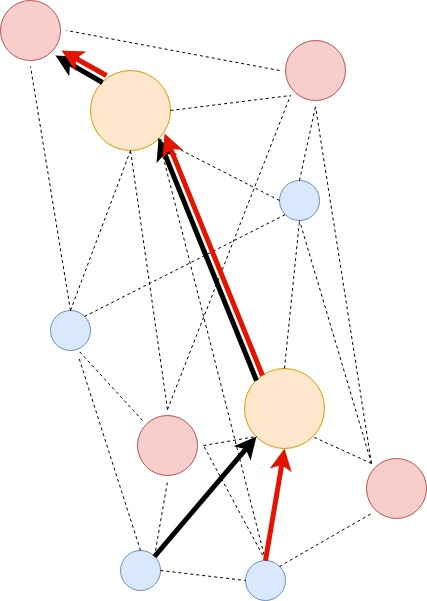
\includegraphics[scale=0.4]{fotos/uniqnuessstisfied.jpg}}
\subfigure[verletzte Leitwegbedingung]{\label{fig:bb}
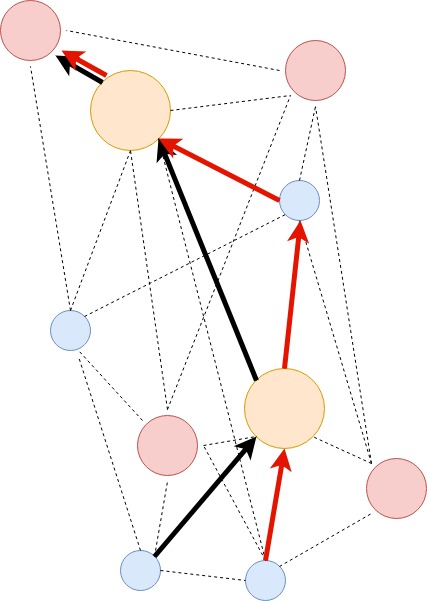
\includegraphics[scale=0.4]{fotos/uniqnuesviolated.jpg}}
\caption{Abbildung der Leitwegbedingung für Routen der zwei Sendungen mit gleichem Ziel}
\end{figure}

\paragraph{Transportzeit.}
Die Sendungen müssen ihr Ziel erreichen, und zwar rechtzeitig. Die Transportzeit bzw. der Zeitraum zwischen der Bereitstellung der Sendung im Quell-Knoten (spezifiziert durch den Parameter „Aufkommenszeitpunkt der Sendung“) und Ankunftszeit am Ziel soll das Zeitlimit, das durch den Parameter „Maximale Transportzeit“ jeder Sendung festgelegt ist, nicht überschreiten. Transportzeit der Sendung besteht aus verschiedenen Komponenten wie der echten Fahrtzeit, der Abfahrt-Bearbeitungszeit und Rangierzeit an den Zwischenbahnhöfen. Außerdem ist eine Wartezeit ggf. vorstellbar, falls eine Sendung zur Bündelung auf andere Sendungen, die noch nicht angekommen sind, in einer Zwischenanlage warten muss. Da die Sendungen Im zeitlichen Modell der Kanten mit konkreten Abfahrtzeiten zugeordnet werden, wird die Wartezeit auch implizit bestimmt.

\paragraph{Zielsetzung des Problems.}
wie schon in \hyperref[subsec:routenplan]{1.1.1} erklärt wurde, das Entscheidungsunterstützungssystem sollte den optimalen Routenplan herausfinden. Zur Optimierung des Routenplans werden die verursachten Kosten minimiert. Jede Lösung präsentiert also einen Routenplan mit der verursachten Kosten als Zielfunktionswert, und kann unter Berücksichtigung der genannten Restriktionen zulässig oder unzulässig sein. Im folgenden sind alle Kostenkomponenten nochmals zusammengefasst:

\begin{itemize}
    \item Zugkosten
    \item Umstellkosten
    \item Richtungsgleiskosten
    \item Anlagenfixkosten
    \item Wagenstundenkosten
    \item Transferzeitkosten
\end{itemize}

Es ist zu beachten, dass ein Routenplan die Zug- bzw. Gleisbelegung nicht explizit aufweist. Trotzdem sollen die Variablen zur Berechnung der Routenplan-Kosten generiert werden. Z.B. die Zugkosten einer Kante lässt sich mit der folgenden Formel rechnen.
\begin{equation*}
    \begin{aligned}
        & e_{ij}^t : \textit{Die Kante von i nach j mit der Abfahrtszeit t} \\
        & \textit{Zugkosten der Kante } e_{ij}^t  = \textit{Anzahl der Züge auf der } e_{ij}^t * \textit{Zugkosten der } e_{ij}^t
    \end{aligned}
\end{equation*}
Um die Anzahl der Züge auf der Kante $e_{ij}^t$ zu bestimmen, wird der Routenplan nach den Routen durchsucht, in denen die Kante $e_{ij}^t$ auftritt. Dementsprechend wird es durch die Summe des Gewichts bzw. der Länge der durchfahrenden Sendungen festgesetzt, wie viele Züge auf der Kante $e_{ij}^t$ benötigt werden. Ähnliches Verfahren wird zur Bestimmung der Knotenbelegung gefolgt, um die Anlagenfixkosten, die Umstellkosten und die Richtungsgleiskosten zu berechnen.\\

Da die Zielfunktion des Problems multikriteriellen Ziele (Kostenkomponenten) beinhaltet, und die Auswirkung jedes Ziels nach Auswertung der Anwender bei verschiedenen Szenarien steuerbar sein sollte, wird außerdem jeder Kostenkomponente eine Gewichtung zugeordnet, und die gewichtete Summe wird im Endeffekt als Zielfunktionswert genommen. Die Gewichtung einigt auch die Kosteneinheiten insbesondere für die Transferzeitkosten und Wagenstundenkosten.

\subsection{Aktueller Lösungsansatz}
\label{sec:current}
Der bestehende Lösungsansatz basiert auf der Dissertation von Dr. Henning \cite{homfeld2012consolidating}. Die von Homfeld bearbeitete Problematik beinhaltet zwar keine regulären Abfahrtzeiten, aber eine zusätzliche Nebenbedingung mehr die sog. „Hierarchie Bedingung“. Diese Restriktion beschränkt den Routenplan je nach den auf Bahnhof-Klassen basierenden Vorschriften. Da die Anlagen sich in Größe und technische Ausstattungunterscheiden, sind bei der Deutschen Bahn die Bahnhöfe in vier Klassen eingestuft: Ebene-0 Rangierbahnhöfe, Ebene-1 Knotenbahnhöfe, Ebene-2 Mittelbahnhöfe und Ebene-3 Anlieferungsbahnhöfe angeordnet.\\

Dementsprechend gibt es zurzeit zwei Ansätze (heuristisch und exakt) für jede Problemstellung (Hierarchie-Modell und Zeit expandiertes Modell). Im folgenden werden die einzelnen Arbeitsschritte zusammengefasst erklärt.

\subsubsection{Graph-Transformation}
Bezüglich der vom Anwender ausgewählten Problemstellung wird zunächst der Verkehrsgraph des Szenarios transformiert. Sind also reguläre Abfahrtzeiten relevant, wird der Graph zeitlich expandiert. Ist aber umgekehrt die Hierarchie-Bedingung wichtig, wird der Verkehrsgraph so transformiert, dass die Hierarchie-Bedingung erfüllt wird.

\paragraph{Zeitliche Expansion.}
Wie schon erwähnt wurde, hat jede Kante täglich reguläre Abfahrtzeiten. Der Graph des Verkehrsnetzwerks des jeweiligen Szenarios wird daher zunächst zeitlich expandiert. Durch die Expansion werden die Kanten und Knoten zeitlich angepasst. Bild 3 zeigt, wie beispielweise die Anlage $A$ und $B$ sowie Kante $AB$ mit täglich 4 Abfahrtzeiten nach der Zeitexpansion darzustellen sind.

\begin{figure}[ht]
\centering
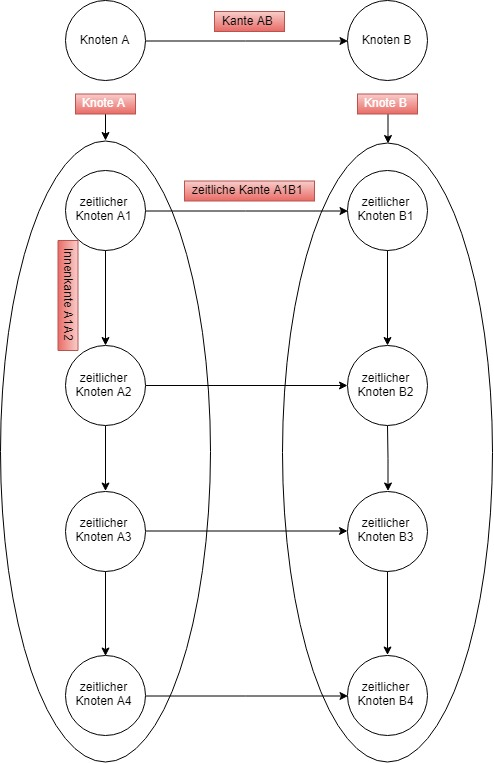
\includegraphics[scale=0.3]{fotos/timeexpansion.jpg}
\caption{Darstellung der Zeitexpansion}
\end{figure}

Da die zeitlichen Knoten $A^{t_i}$ und $B^{t_j}$ sowie die zeitlichen Kanten $AB^{t_i} $ ($t_i$ bezeichnet die Abfahrtzeit der Kante) nur die Zeitkomponenten des ersten Tages abbilden, werden die zeitliche Knoten und Kanten in den folgenden Tagen des Planungshorizonts ausgerollt. Die maximale Transportzeit in der Menge der Sendungen wird als den Planungshorizont angenommen. Die räumliche Knoten $A$ und $B$ sowie die Kante $AB$ bekommen also nach der Expansion die Zeitkomponenten $A^{t_i, m. Tag}$ , $B^{t_j, m. Tag}$ und $AB^{t_i, m. Tag}$. $AB^{t_i, m. Tag}$ bezeichnet also die Kante $AB$, die am Tag $m$ um $t_i$ abfährt.\\

falls es an der A und B Knoten noch weiteren Abfahrten gäbe, würden dementsprechend mehrere Zeitliche Knoten und Kanten erzeugt.

\subsubsection{Heuristischer Lösungsansatz}
Der heuristische Ansatz vorgeschlagen von \cite{homfeld2012consolidating} und basierend auf dem Fluss-Model „Rip-up and Reroute“ versucht, erstmals eine Initiallösung zu erzeugen. Danach werden die Routen einiger Sendungen vom Initial-Routenplan ausgenommen und wieder geroutet. Der vorherige Schritt wird iterativ fortgesetzt, sobald das Terminierungskriterium getroffen wird.

\subsubsection{Mathematische Modellierung}
Schließlich wird ein MIP-Model mit den verschiedenen Entscheidungsvariablen er-stellt. Die drei wichtigsten Entscheidungsvariablen sind die Flussvariablen sowie Zugvariablen und Richtungsgleis-Variablen. Zur Modellierung der Leitwegbedingung wird eine zusätzliche Entscheidungsvariable, die sog. „Baumvariable“ hinzugefügt. Sind ungeroutete Sendungen erlaubt, wird dazu jeweils eine Entscheidungsvariable definiert.\\
Anhand eines MIP-Solvers (Gurobi oder Cplex) wird das Model schließlich gelöst. Die beste heuristische Lösung kann dem MIP-Solver als Initiallösung eingegeben werden.\\
Es wurde wie beschrieben jeder Kostenkomponente eine Gewichtung zugeordnet. Damit kann man die Auswirkung der Kostenbestandteile jeweils beliebig verstärken oder sogar komplett ausschalten, falls die Gewichtung gleich null gesetzt wird. Das Problem bei den unterschiedlichen Kosteneinheiten wurde mithilfe eines Faktors behoben, der Zeit-Einheit in Geld-Einheit umwandelt.


\section{Zielsetzung dieser Arbeit}
\label{sec:Ziel}
Die Zeitexpansion vergrößert rasant den räumlichen Verkehrsgraphen, und erzeugt viele zeitlichen Knoten und Kanten, worauf aber der jetzige heuristische Lösungsansatz \emph{(Rip-up and Reroute)} nicht gut reagiert. Sogar mit langer Rechenzeit und tausenden Iterationen fällt normalerweise eine relativ große Lücke zwischen dem besten gefundenen Zielfunktionswert von R\&R und dem MIP-Solver als angewandter exakter Lösungsansatz auf.\\
Nach der Besprechung mit den Fachexperten der Deutschen Bahn sowie dem Lehrstuhl, dem diese Arbeit vorgelegt wird, also Wirtschaftsinformatik insb. Operations Research der Universität Paderborn, wurde die Implementierung und durch diese Abschlussarbeit Dokumentation eines pfad-basierten heuristischen Lösungsansatzes für die beschriebene Problemstellung als Ziel ausgewählt.


%\section{Vorgehensweise}

\chapter{Stand der Forschung}
Dieses Kapitel beschäftigt sich mit der vorhandenen Fachliteratur bezüglich der beschriebenen Problemstellung.
\section{\textit{„block“} und \emph{„blocking problem“}}
Die Optimierung des Güterverkehrssystems interessiert die Forscher schon lange. Die beschriebene Problemstellung ist in der Literatur unter dem englischen Begriff bzw. Stichwort \emph{„blocking problem“} zu recherchieren. In Bezug auf den technischen Aspekt sowie die Modellierung unterscheidet sich diese Arbeit aber von vielen Aufsätzen durch die Definition von \textit{„block“}. Bei der Erstellung einer Blockkante zwischen zwei Anlagen wird in vielen Aufsätzen eine direkte Verbindung zwischen den beiden Stationen hergestellt. Beispielsweise die kontinuierliche Entscheidungsvariable  \(x_{ijkp}\)  in \cite{bodin1980model} deutet darauf hin, wie viele Eisenbahnwaggons vom Bahnhof \(i\) im \(j\) umgestellt werden, welche durch \(p.\) Pfad an den Bahnhof \(k\) landet. Ein Wagon im Bahnhof $i$, das den Bahnhof $k$ als Ziel-Knoten hat, wird also als nächstes zur Umstellung in dieser Blockkante zum Bahnhof $j$ transportiert. Die Blockkante vom $i$ bis zum $j$ ist eigentlich ein Bestandteil der Sendungsroue $p$, die an $k$ endet. Im Allgemeinen verlässt bei $j=k$ ein Wagon das Optimierungssystem.\\
Im Gegensatz dazu und angepasst an die Voraussetzungen der Deutschen Bahn, bedeutet eine Blockkante bei \cite{homfeld2012consolidating} eine Gruppe der Waggons, die in Züge aufgeteilt wird. Die Züge auf eine Blockkante haben zwei Kapazitätsrestriktionen (nach dem Gewicht und der Länge). Das Einsetzen von mehr als einem Zug pro Kante ist außerdem auch erlaubt \textit{(vgl. \cite{homfeld2012consolidating})}. In dieser Arbeit wurde Homfelds Konzept der Blockkante so erweitert, dass die Kanten die konkrete Zeitkomponenten bzw. Abfahrt- und Ankunftszeit sowie Wartezeit auch explizit aufweisen.\\

\section{„Fluss-Model“ und „Pfad-Model“}
Allgemein kann jedes \textit{„blocking problem“} als ein Grundmodel \textit{„Multi-commodity capacitated network design problem“} (MCNDP) mit zusätzlichen Entscheidungsvariablen sowie Nebenbedingungen betrachtet werden. Das Model lässt sich mathematisch mit zwei Formulierungen, nämlich das „Fluss-Model“ \textit{(auf engl. arc-based)} und das „Pfad-Model“ \textit{(auf engl. path-based)} , interpretieren. Für Details zu mathematischen Formulierungen wird auf die Aufsätze \cite{hewitt2010combining} und \cite{frangioni20090} verwiesen. Die beschriebene Problemstellung hat dementsprechend auch zwei Formulierungen. \cite{homfeld2012consolidating} hat die Formulierungen sowie das Dual-Problem und Ungleichungen in Bezug auf das Hierarchie-Model aufgebaut.\\

\section{In der Literatur vorgeschlagene Lösungsansätze}
Für das {„blocking problem“} sowie das Grundmodel \textit{„Multi-Commodity capacitated Network design Problem“} wurden in der Literatur verschiedene exakte bzw. heuristische Lösungsansätze vorgeschlagen. Wegen der exponentiell steigenden Anzahl der Entscheidungsvariablen bei der Pfad-Formulierung wurden vor allem die auf \textit{„Column Generation“} basierende Methoden angewendet. \cite{barnhart2000railroad} bietet einen heuristischen Ansatz basierend auf \emph{„lagrangian relaxation“} für das als Fluss-Model formulierte blocking-Problem an. Der Zerlegungsverfahren teilt das komplexe MIP-Model in zwei Unterprobleme auf. Einige Ungleichungen werden zu dem Teilproblem hinzugefügt, um die unteren Schranken zu verschärfen und die Erzeugung der Lösungen zu erleichtern. Die Subgradienten-Optimierung wird auch zur Lösung des Lagrangian Dual-Problems verwendet.\\
\cite{hasany2018modeling} haben ebenfalls eine Heuristik basierend auf dem Dekomposition-Algorithmus entwickelt, der das linearisierte Modell in zwei einfachere und unabhängige Unterprobleme unterteilt. Das erste Unterproblem zielt darauf ab, die beste Route für die Güterwagen zu finden. Die Route erfüllt die Fluss- sowie Nachfragebeschränkungen. Das zweite aber ermittelt für den Pfad, den das erste Unterproblem erzeugt hat, die optimale Anzahl der durch einzelne Blockkanten fahrenden Züge. Weil manche Restriktionen durch Zerlegungsverfahren relaxiert werden, kann dieser Ansatz die Zulässigkeit der generierten Lösung nicht gewährleisten.\\
\cite{crainic2000simplex} schlagen eine Simplex-basierte Tabu-Suchmethode für das MCNDP vor, indem sie eine auf dem Pfad-Model basierende Problemformulierung verwenden. Ihre Methode kombiniert die Spaltengenerierung mit Pivot-artigen Bewegungen einzelner Sendungsflüsse, um im Endeffekt die Pfadflussvariablen zu bestimmen.\\
\cite{ghamlouche2003cycle} stellen eine zyklusbasierte Nachbarschaft zur Anwendung in einem metaheuristischen Lösungsansatz für MCNDP dar. Die Hauptidee der zyklusbasierten lokalen Verschiebungen steckt in der Umleitung der Güterflüsse in Zyklen, um vorhandene Kanten aus dem Netzwerk zu entfernen und durch neue Kanten zu ersetzen. In \cite{ghamlouche2004path} erweitern sie die Anwendung der neuen Nachbarschaft in einem evolutionären Algorithmus. Ihr Rahmenkonzept basiert auf \emph{„Pfad-Relinking“}, was bezüglich der \emph{„Scatter-Suche“} für evolutionäre Algorithmen ursprünglich in \cite{glover1998template} vorgeschlagen wurde. Die zyklusbasierte Nachbarschaft erzeugt eine Elite-Kandidatenmenge der Lösungen durch einen Tabu-Suchalgorithmus, welche als Rekombinationsmethode zur Erzeugung der Nachkommen funktioniert. Bei Aktualisierung des Lösungspools wird die Unähnlichkeit der Lösungen als zusätzliche Komponente bei der Berechnung des Zielfunktionswerts betrachtet.\\
\cite{alvarez2005scatter} schlagen ebenfalls eine Version des Scatter-Suchalgorithmus für MCNDP vor, indem der von \cite{feo1995greedy} vorgestelltem \emph{GRASP} \emph{(auf engl. greedy randomized adaptive search procedure)} zur Herstellung eines diversifizierten initialen Lösungspools angewendet wurde. Beim nächsten Schritt werden verschiedene kombinierte Untermengen aus den Sendungspfaden im Lösungspool erstellt. Dann aus jeder Untermenge werden die besten Pfade für ein Verbesserungsverfahren ausgewählt. Ein Zulässigkeitsmechanismus ist auch zuständig, um die unzulässig generierten Lösungen wiederherzustellen. Im Gegensatz dazu betrachtet die Scatter-Suche von \cite{paraskevopoulos2016cycle} die Sendungspfade zur Rekombination der Lösungen zum Erzeugen der Nachkommen nicht. Stattdessen werden die Kanten aus einer Untermenge der Lösungen kombiniert. Sie beanspruchen, dass diese Modifikation die Leistung des Scatter-Suchalgorithmus verbessert, weil damit mehr Varianten durchsucht werden können, was zu einem diversifizierten stärkeren Pool der Nachkommen führt. Eine iterative Methode zur lokalen Suche ist dann für die Verbesserung einzelner der Nachkommen zuständig, indem  eine Heuristik die binären Variablen bezüglich der Kantenbelegung festsetzt, und dann ein MIP-Model zur Bestimmung der Flussvariablen oder Unzulässigkeit der festen Kanten aufgebaut wird. Ein zyklusbasierter Nachbarschaft-Operator ermöglicht vollständige oder teilweise Umleitung mehrerer Güter. 


\chapter{Lösungsansatzvorschlag}
Hinsichtlich des mathematischen Pfad-Models besteht die Optimalität in der besten Kombination aus den möglichen Pfaden. Daher wird wegen untrennbarer Sendungen jeder Sendung ein bloßer Pfad so zugeordnet, dass der Routenplan aus den Pfaden die minimalen Kosten bezüglich der entgegengesetzten Ziele (wie Schnelligkeit und Bündelungseffekt) aufweist.\\
Wegen der exponentiell steigenden Anzahl der Pfad-Variablen wurde in der Literatur oft die auf Spaltengenerierung basierenden Methoden angewendet. wenn das Szenario also \(n\) Sendungen umfasst, und die Sendung \(i\) eine Anzahl von \(k_i\) Pfade besitzt, hat der Lösungsraum $\prod\limits_{i=1}^n k_{i}$ verschiedene Möglichkeiten. Trotzdem stehen nur \(n\) Pfade in der Basis jeder Simplex-Tableau (Lösung). Deshalb kann man zuerst durch eine Initial-Lösung viele Pfade vernachlässigen, und dann iterativ die Pfade (Spalten) mit der potenziellen Verbesserung der Basis hinzufügen.\\
\cite{homfeld2012consolidating} stellt zwar Anhand der mathematischen Formulierung des dualen Problems eine Formel für den Pricing-Schritt der Spaltengenerierung vor, die mit den aktuellen dualen Variablen sowie den Parameter bezüglich der Kanten und Anlagen verbunden ist, aber ist es im Vergleich zu der Pricing-Formel eines klassischen \emph{Multi-Commodity flow model} komplexer, da die Blockprobleme prinzipiell mehr Restriktionen und entsprechend mehr duale Variablen beinhalten. Aus diesem Grund versuchen wir in dieser Arbeit, statt der expliziten Rechnung der dualen Variablen und der daraus gerechneten reduzierten Werten die kompetitiven Pfade durch Effizienz-Verhältnisse wie Zugauslastung zu ermitteln.\\
Mit der Inspiration des Dekomposierungsverfahrens zerlegen wir das Problem in zwei einfachere Unterprobleme. Wir versuchen dabei erstmals, aus den günstigeren Einzel-Pfaden (in Bezug auf Distanz bzw. Reisezeit) eine Kombination zu bestimmen. Dafür bauen wir einen evolutionären Algorithmus anhand des Rahmenkonzepts der Scatter-Suche auf. Da die durch Preprocessing generierten Pfade aus den Kanten mit den frühesten Abfahrtzeiten bestanden sind, soll im zweiten Schritt die Abfahrtzeit der Kanten aus den festen Pfaden, die durch erstes Unterproblem erzeugt worden sind, angepasst werden. \\

\section{Preprocessing-Schritt}
Das Ziel des Preprocessingsverfahrens besteht darin, alle zulässigen Pfade jeder Sendung zu erzeugen, die als Input zur Erstellung der Entscheidungsvariablen eines Pfad-basierten Algorithmus einzugeben sind. Der betroffene Graph des Szenarios sowie die Liste aller Sendungen sind ursprünglich diesem Schritt als Input einzugeben. Es gibt drei Einschränkungen, die die Zulässigkeit eines Pfades bestimmen. Strukturbeschränkung ist zuerst zu nennen, d.h. je nach Graph, ob die Reihenfolge der Knoten und Kanten bzw. der Pfad zulässig ist. Die maximale Transportzeit sowie die maximale Anzahl der Umstellungen sind auch für die Zulässigkeit eines Pfades entscheidend. Sie beziehen sich auf das Input bezüglich der Sendungen.\\

Die klassische Tiefensuche \emph{(auf engl. Depth first search algorithm)} ist ein Algorithmus zum Durchqueren bzw. Durchsuchen der Graph- oder Baum-Datenstrukturen. Die Anwendung dieses Algoritmus ist jedoch mit Herausforderungen verbunden. Einerseits zur Überprüfung der Zulässigkeit eines Pfades nach der maximalen Transportzeit soll der Zeit expandierte Graph durchsucht werden, da dieser Graph die konkreten Abfahrtzeiten und die daraus berechneten Wartezeiten aufweist. Bei den Szenarien aus dem Schienenverkehr sind normalerweise die Wartezeit im Vergleich zu der Transferzeit (reiner Transfer im Zug) besonders dominant. Die Überprüfung der Zulässigkeit nach der Transferzeit allein, was nach dem räumlichen Graphen ebenfalls zu ermitteln ist, ist daher nicht versprechend. Auf der anderen Seite ist aber die Suche durch den Zeit expandierten Graphen wegen der Komplexität sehr viel rechenaufwändiger als beim räumlichen Graphen.\\

Als Lösung schlägt diese Arbeit eine spezielle Version der Tiefensuche vor, die ein vereinfachtes Exemplar des räumlichen Graphen nach den strukturell zulässigen Pfaden sucht. Zur Überprüfung der Zulässigkeit nach der maximalen Transportzeit wird trotzdem der expandierte Graph nach der Kante mit der frühesten zulässigen Abfahrtzeit durchsucht. Somit erreicht die Tiefensuche im Endeffekt einen Pfad aus den Kanten mit den frühesten Abfahrtzeiten. Dann wird die Zeitspanne zwischen der Ankunftszeit am Ziel für diesen Pfad (die früheste Ankunftszeit basiert auf Transport mit diesem Pfad) und der spätesten Ankunftszeit (basiert auf maximaler Transportzeit der Sendung) gerechnet. 
Die späteren aber noch zulässigen Zeitlichen Kanten lassen sich diese Zeitspanne entsprechend auch generieren. Anhand eines rekursiven Aufrufs läuft der Algorithmus weiter, sobald er alle zulässigen Pfade herausfindet.

\section{Heuristisches Verfahren zur Einstellung der Abfahrtzeiten}
Jede Pfad-Kombination besteht aus den Pfaden mit frühesten Abfahrtzeiten einzelner Sendung, welche die Tiefensuche durch den Preprocessing-Schritt erzeugt.  Die Tiefensuche stellt auch sicher, dass alle Pfade bezüglich der maximalen Transportzeit und maximallen Anzahl der Umstellungen zulässig sind, und generiert auch die noch zulässige Verschiebungsmöglichkeiten für jede Kante einzelnes Pfades. Trotzdem ist zur Erstellung eines Routenplans aus der Kombination die Bestimmung der Abfahrtzeitzeit der Kanten ebenfalls notwendig. Sonst würden die Sendungen trotz der gleichen räumlichen Kanten schließlich nicht gebündelt. Aus diesem Grund würden die Abfahrtzeit der Kanten aus festen Pfaden hier eingestellt, d.h. die Frage im diesen Unterproblem besteht darin, ob es sich lohnt, eine \(A\to B\) Kante eines Sendungspfads zu verschieben, damit die Sendung mit anderen Sendungen, deren Pfad auch die \(A\to B\) Kante mit verschiedener Abfahrtzeit umfasst, konsolidiert wird. In anderen Worten formuliert, soll zwischen die Ersparnis durch Bündelungseffekt und die schnellere Routen mit gleichen räumlichen Knoten und Kanten ein Kompromiss festgesetzt werden.\\



\section{Evolutionärer Algorithmus zur Optimierung der Pfad-Kombination}
Anhand einer Scatter-Suche und Rekombination-Methode versuchen wir die Vielfältigkeit bzw. Exploration zu erhöhen. Im Gegensatz dazu fokussiert eine heuristische lokale Nachbarschaft-Suche auf das lokale Optimum, und versucht jede Lösung aus dem Pool unter einem gewissen Nachbarschaft zu verbessern. Für Rekombinationsmethode kan die methode \emph{"path relinking"} vorgeschtelt von \cite{glover2003scatter} angewendet werden.\\
\todo{Read scatter search and path relinking}
\chapter{Konzept}

\section{Subgradientenverfahren}
Das \emph{Subgradientenverfahren} wurde von \cite{HeKa71} \todo{verify} vorgeschlagen um das duale Lagrange Problem (LDP) approximativ zu lösen. Das Verfahren ist iterativ, dabei wird in jeder Iteration zuerst das Lagrange Problem $Z_D(\mu)$ für gegebene Multiplikatoren $\mu$ gelöst und im zweiten Schritt neue Multiplikatoren für die nächste Iteration berechnet. Das ganze wird wiederholt bis eine Abbruchbedingung erfüllt ist.
\begin{algorithm}
	\label{subgradientenverfahren}
	\caption{Das Subgradientenverfahren}
	Initialisiere $\mu^0$\\
	Iterationszähler $k$ = 0\\
	Berechne obere Schranke $Z^*$ (evtl. heuristisch)\\	
	\While{Keine Abbruchbedingung erfüllt} {
		Löse Lagrange Relaxation $Z_D(\mu^k), x^k$ ist die optimale Lösung\\
		Berechne Subgradient-Vektor $s^t = b - Ax^k$\\
		Berechne Suchrichtung $d^k$ \\
		Berechne Schrittweite $t^k$ \\
		Aktualisiere Multiplikatoren $\mu^{k+1} = \mu^k + t^k d^k$\\
		$k = k + 1$\\
	}
\end{algorithm}

Algorithmus \ref{subgradientenverfahren} beschreibt die Grundstruktur des Verfahrens. Die entscheidenden Faktoren, die die Performanz des Verfahrens und die Lösungsqualität bestimmen, sind die Berechnung der Suchrichtung $d^k$ und der Schrittweite $t^k$ sowie die Abbruchbedingungen. Diese Aspekte sollen im weiteren genauer erläutert werden.

\section{departure Time heuristic adjuster}



\(ref\) Kantenergebnisse-Referenz

\begin{algorithm}
	\label{Abfahrtszeit-Einsteller}
	\caption{Heuristischer Abfahrtszeit-Einsteller}
	\KwIn{die Pfad-Kombinationen mit frühesten Abfahrtzeiten\((k_i , p_i^{t_{min}})\)}
	\KwOut{optimaler Routenplan \(RP(k_i , p_i^{t^*})\)}
	$ RP \gets$ initialisiere mit \((k_i , p_i^{t_{min}})\)\\
	\For{jede Kombination \(k_i , p_i\) aus Input}{$ ref \gets Aggregation(k_i , p_i^{t_{min}})$ }
	\While{\(ref\) enthält eine Kante mit Verschiebungspotential}
	{
    	$L \gets$ initialisiere eine neue Verschiebungsiste\\
	    Kandidatenkante \(er_{ij}^{t_m} \gets\) erste Kante mit Verschiebungspotential\\auf \(t_n\) (maximal vorkommende Abfahrtzeit) aus \(ref\)\\
        \If{\(e_{ij}^{t_n} \) ist für die durchfahrende Sendungen auf  \(e_{ij}^{t_m} \) zulässig}{
        	\(k_i \gets\) die durchfahrende Sendungen auf  \(e_{ij}^{t_m} \)\\
            aktualisiere VerschiebungsListe \(L \gets k_i , e_{ij}^{t_m}  , t_n\)\\
            \(Tiefensuche Der Sendungspfade( L )\)\\
            \(VerschiebungUndEvaluierung(L)\)\\
       }  
	}
\end{algorithm}

\begin{algorithm}
	\label{TiefensuchePfad}
	\caption{Tiefensuche Der Sendungspfade}
	\KwIn{Untermenge der Verschiebungsliste (neue Verschiebungsaufträge) $L_n$}
	\For{jede Verschiebung \(k_i , e_{ij}^{t_m}  , t_n\) aus $L_n$}
	{
	    $p_k \gets$ aktuell optimaler Pfad der Sendung $k_i$ aus $RP$\\
        $t_i^n \gets$ maximal zulässige Abfahrtzeit aller Kanten der $p_k$ nach $e_{ij}^{t_n}$\\
	    \For{jede Kante $e_{lm}^{t_r}$ aus $p_k$}
	    {
	        \If{$e_{lm}$ ist $e_{ij}$}{setze fort}
	        
	        $er_{lm}^{t_r} \gets$ hole das gemappte Kantenergebnis aus $ref$\\
	        
	        \If{versuche alle durchfahrende Sendungen in $er_{lm}^{t_r}$ auf ein spätere Zeitpunkt bis zum maximal $t_l^n$ zu verschieben}
	            {
	                \If{neue Verschiebungszeitpunkt $< t_l^n$}
	                {initialisiere die neue Verschiebungsliste}
	                
	                $L_n \gets$ neue Verschiebungsaufträge\\
	                $Tiefensuche Der Sendungspfade( L_n )$\\
	            }
	    }
	}
\end{algorithm}

versuche alle durchfahrende Sendungen in $er_{lm}^{t_r}$ auf ein spätere Zeitpunkt bis zum maximal $t_l^n$ zu verschieben
%\chapter{Ergebnisse}

\begin{table}[h]
\begin{tabular}{lccccccc}

{\bf Problem} & {\bf Dienste} & {\bf Busse} &   {\bf LB} &   {\bf UB} & {\bf Zeit} & {\bf Spalten CSP} & {\bf Fixierung} \\
\hline
    320A01 &         54 &         25 &     79.333 &     86.418 &   05:32:44 &    100.000 &            \\

    320A03 &         54 &         24 &     79.178 &     86.184 &   07:03:14 &    120.586 &            \\

    320A05 &         40 &         20 &     62.981 &     66.166 &   06:02:23 &    100.000 &            \\

    320A07 &         58 &         27 &     85.927 &     92.968 &   06:26:15 &    178.231 &            \\

    320A09 &         54 &         25 &     81.758 &     87.568 &   06:10:01 &    167.585 &            \\
\hline
           &   {\bf 52} & {\bf 24,2} & {\bf 77.835} & {\bf 83.861} & {\bf 06:14:55} & {\bf 133.280} &     {\bf } \\

\end{tabular}
\caption{Verfahren von Huisman für ausgewählte ECOPT-Instanzen mit 4 Depots und 320 Servicefahrten, Variante A}.
\end{table}

\chapter{Zusammenfassung und Ausblick}
Zusammenfassende Würdigung der Ergebnisse, Fazit und Ausblick

\bibliography{bibliography} % Literaturverzeichnis

%\appendix

\chapter{Detaillierte Ergebnisse} \label{tables}


\begin{ergebnisse} \centering	
% Table generated by Excel2LaTeX from sheet 'Tabelle1'
\begin{tabular}{lccccccc}

{\bf Problem} & {\bf Dienste} & {\bf Busse} &   {\bf LB} &   {\bf UB} & {\bf Zeit} & {\bf Spalten CSP} & {\bf Fixierung} \\
\hline
    320A01 &         54 &         25 &     79.333 &     86.418 &   05:32:44 &    100.000 &            \\

    320A03 &         54 &         24 &     79.178 &     86.184 &   07:03:14 &    120.586 &            \\

    320A05 &         40 &         20 &     62.981 &     66.166 &   06:02:23 &    100.000 &            \\

    320A07 &         58 &         27 &     85.927 &     92.968 &   06:26:15 &    178.231 &            \\

    320A09 &         54 &         25 &     81.758 &     87.568 &   06:10:01 &    167.585 &            \\
\hline
           &   {\bf 52} & {\bf 24,2} & {\bf 77.835} & {\bf 83.861} & {\bf 06:14:55} & {\bf 133.280} &     {\bf } \\

\end{tabular}  
\caption{Verfahren von Huisman für ausgewählte ECOPT-Instanzen mit 4 Depots und 320 Servicefahrten, Variante A}.
\end{ergebnisse}

\chapter{Inhalt der CD}

\begin{description}
	\item \textbf{diplomarbeit.pdf} ist dieses Dokument im PDF Format,
	\item \textbf{report/} enthält die \LaTeX-Quellen zu dieser Arbeit,
	\item \textbf{docs/} enthält Zitierte Arbeiten, soweit elektronisch vorhanden,
	\item \textbf{ergebnisse.xls} ist eine Übersicht der Ergebnisse in Tabellenform,
	\item \textbf{test/} enthält Quellen und detaillierte Ausgaben der Experimente:
	\begin{description}
		\item \textbf{src/} enthält den Quellcode der entwickelten Software,
		\item \textbf{logs/} enthält die Ausgabedateien der durchgeführten Experimente,
		\item \textbf{config/} enthält die Konfigurationsdateien der durchgeführten Experimente,
		\item \textbf{instances/} enthält die Probleminstanzen der durchgeführten Experimente.
	\end{description}
\end{description} % Anhänge

\end{document}
